\documentclass[aspectratio=169]{beamer}
\useoutertheme[progressbar=frametitle]{metropolis}
\useinnertheme{metropolis}
\definecolor{nabgray}{rgb}{0.6,0.59,0.61}
\usecolortheme[named=nabgray]{structure}
\usepackage{tikz}
\usepackage[utf8]{inputenc}
\usepackage[spanish]{babel}
\usepackage{fontspec}
\setmonofont{JetBrains Mono}
\setmainfont{Roboto}
\setsansfont{Roboto}

\usepackage{smartdiagram}
\usepackage{qtree}
\usepackage{verbatim}
\usepackage{svg}
\usepackage{graphicx}
\usepackage{color}
\definecolor{lightgray}{rgb}{0.95, 0.95, 0.95}
\definecolor{darkgray}{rgb}{0.4, 0.4, 0.4}
\definecolor{ocherCode}{rgb}{1, 0.5, 0} % #FF7F00 -> rgb(239, 169, 0)
\definecolor{blueCode}{rgb}{0, 0, 0.93} % #0000EE -> rgb(0, 0, 238)
\definecolor{greenCode}{rgb}{0, 0.6, 0} % #009900 -> rgb(0, 153, 0)

\usepackage{upquote}
\usepackage{listings}
\lstset{language=java,
    otherkeywords={var,record},
	% Basic design
	backgroundcolor=\color{lightgray},
	basicstyle={\small\ttfamily},
	frame=l,
	keywordstyle=\footnotesize\color{blue},
	escapeinside={<@}{@>},
	breaklines=true,
	% Line numbers
	xleftmargin={0.75cm},
	numbers=left,
	stepnumber=1,
	firstnumber=1,
	numberfirstline=true
	% Code design
	identifierstyle=\color{black},
	keywordstyle=\color{ocherCode}\bfseries,
	ndkeywordstyle=\color{greenCode}\bfseries,
	stringstyle=\color{ocherCode}\ttfamily,
	commentstyle=\color{darkgray}\ttfamily,
	tabsize=2,
	showtabs=true,
	showspaces=false,
	showstringspaces=false,
	extendedchars=true,
	breaklines=true
}

\lstdefinelanguage{bash}{
    basicstyle=\ttfamily,
    showstringspaces=false,
    commentstyle=\color{red},
    keywordstyle=\color{blue},
    numbers=right,
    xleftmargin={0.25cm}
}

\usebackgroundtemplate
{
	
\includegraphics[width=\paperwidth]{Images/fondo}%
}


\title{Tolerancia a fallas, service mesh y chassis}
\author{Víctor Orozco - @tuxtor}
\institute{Nabenik}
\date{\today}

\begin{document}

{
    \usebackgroundtemplate{
\includegraphics[width=\paperwidth]{Images/portada}}
    \setbeamercolor{frametitle}{fg=red}
    \usebeamercolor[fg]{normal text}
    \frame{\titlepage}
}



\begin{frame}{}
    \begin{figure}
        \centering
        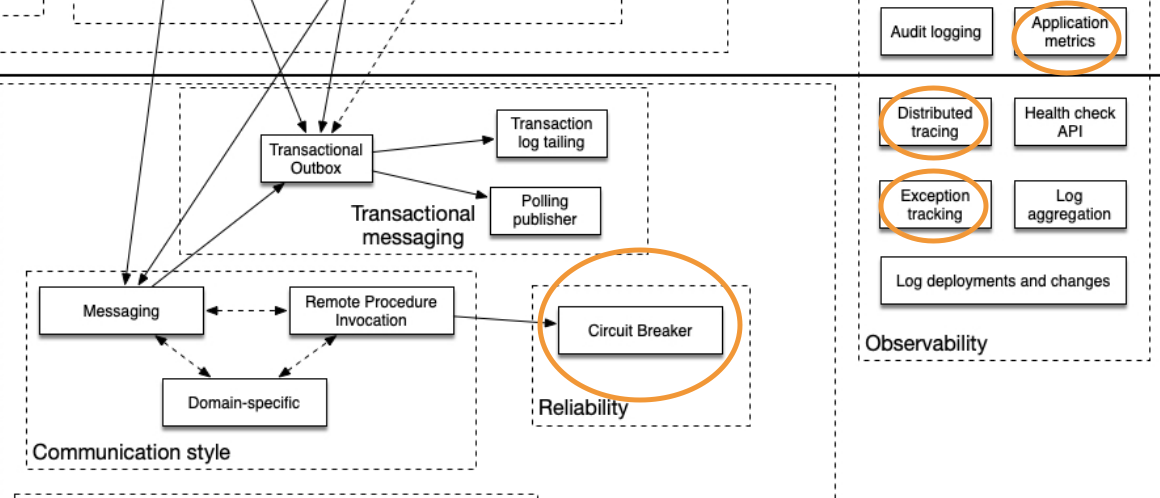
\includegraphics[width=\linewidth]{Images/patterns.png}
    \end{figure}
    Fuente: \url{https://microservices.io}
\end{frame}

\begin{frame}{}
    \begin{figure}
        \centering
        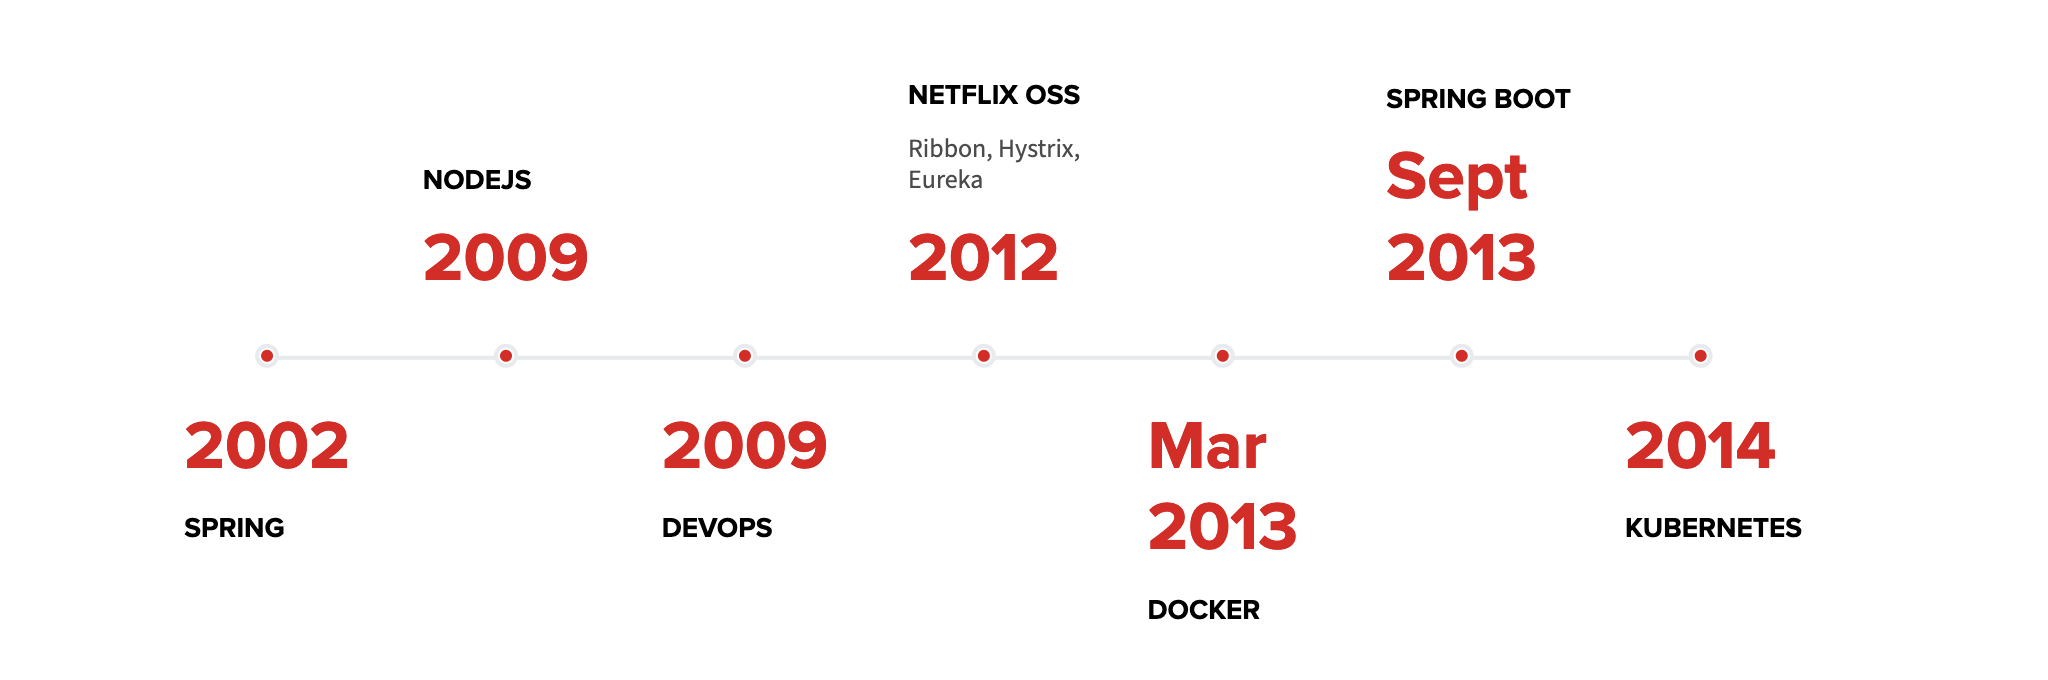
\includegraphics[width=\linewidth]{Images/evolucioncloudnative.png}
    \end{figure}
\end{frame}


{
    \usebackgroundtemplate{
\includegraphics[width=\paperwidth]{Images/separador}}
    \setbeamercolor{normal text}{fg=white}
    \setbeamercolor{frametitle}{fg=red}
    \usebeamercolor[fg]{normal text}
    \section{Tolerancia a fallas vía chassis}
}


\begin{frame}{}
    \begin{figure}
        \centering
        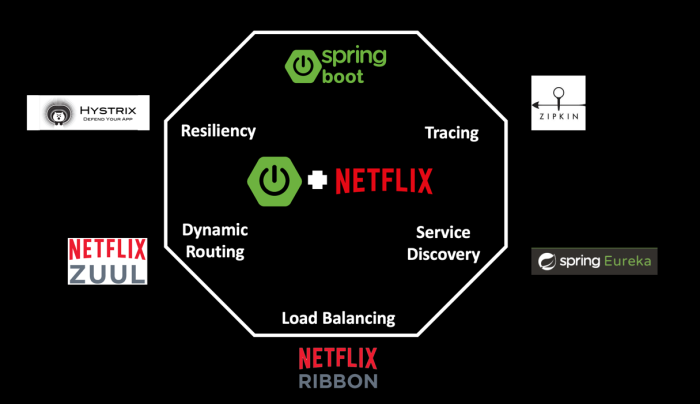
\includegraphics[width=\linewidth]{Images/netflix.png}
    \end{figure}

\end{frame}




\begin{frame}{Fault Tolerance + Metrics}


\begin{figure}
	\centering
	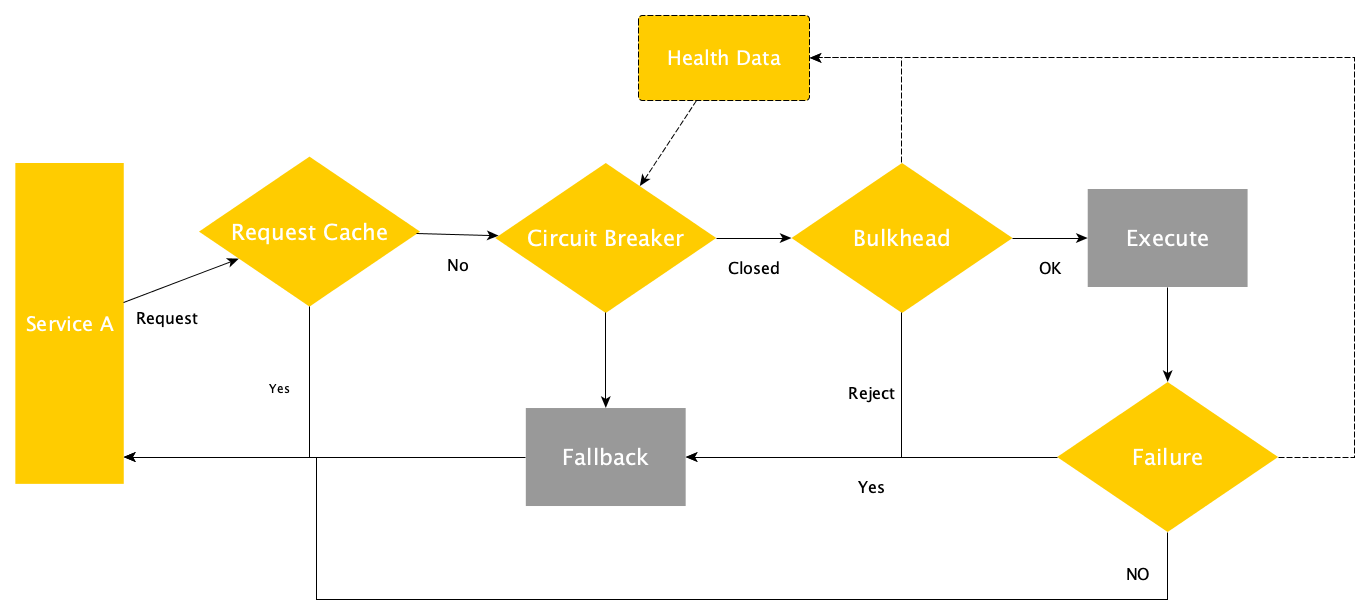
\includegraphics[width=0.9\linewidth]{Images/falldata}
\end{figure}

\end{frame}


\begin{frame}{Stack sin kubernetes}


Java
\begin{itemize}
\item Tolerancia a fallas: Hystrix, Resilence4j, MicroProfile Fault Tolerance
\item Metricas: Spring Metrics, Micrometer, MicroProfile Metrics
\end{itemize}


Node
\begin{itemize}
\item Tolerancia a fallas: Opposum
\item Metricas: prom-client
\end{itemize}


Consumidor: OpenMetrics (Prometheus)
\end{frame}


\begin{frame}{Fault tolerance}

Reglas comunes
\begin{itemize}
\item Circuit Breaker
\item Bulkhead
\item Retry
\item Timeout
\item Fallback
\end{itemize}

\end{frame}

\begin{frame}[fragile]{Fault tolerance - Fallback, Timeout}
\begin{lstlisting}
@GET
@Path("/{id:[a-z]*[0-9][0-9]*}")
<@\textcolor{red}{@Fallback(fallbackMethod = "findByIdFallBack")}@>
<@\textcolor{red}{@Timeout(TIMEOUT)}@>
public Response findById(@PathParam("id")
final String imdbId) {
...
}

public Response findByIdFallBack(@PathParam("id")
final String imdbId) {
...
}
\end{lstlisting}
\end{frame}



{
    \usebackgroundtemplate{
\includegraphics[width=\paperwidth]{Images/separador}}
    \setbeamercolor{normal text}{fg=white}
    \setbeamercolor{frametitle}{fg=red}
    \usebeamercolor[fg]{normal text}
    \section{Tolerancia a fallas vía orquestador}
}

\begin{frame}{Tolerancia a fallas}

    \begin{block}{Caracteristicas chassis}
        \begin{itemize}
            \item Dependiente de plataforma
            \item Basado en interceptores
            \item Tooling overhead
        \end{itemize}
    \end{block}

\end{frame}

\begin{frame}{Kubernetes}

    \begin{exampleblock}{¿Que es Kubernetes?}
        \begin{itemize}
            \item Orquestador
            \item Gestiona aplicaciones y despliegues (en contenedores)
            \item Declarativo
            \item Elastico (scale up)
            \item \textbf{Resiliente (self healing)}
            \item Actualizaciones
        \end{itemize}
    \end{exampleblock}
Kubernetes por si mismo \textbf{no hace los servicios tolerantes a fallas entre llamadas}
\end{frame}


\begin{frame}{Service mesh}


\begin{columns}[T] % contents are top vertically aligned
\begin{column}[T]{7cm} % each column can also be its own environment
\begin{alertblock}{¿Que es un Service Mesh?}
        \begin{itemize}
            \item Interceptores a nivel de red (Proxy)
            \item Sidecar dentro de pods
            \item Independiente de lenguaje de programación
            \item Gestión de comunicación de servicios
            \item Observabilidad
            \item \textbf{Tolerancia a fallas}
           \item Chaos Engineering
            \item Istio, Linkerd, Conduit
        \end{itemize}
    \end{alertblock}
\end{column}
\begin{column}[T]{5cm} % alternative top-align that's better for graphics
	\begin{figure}
		\centering
		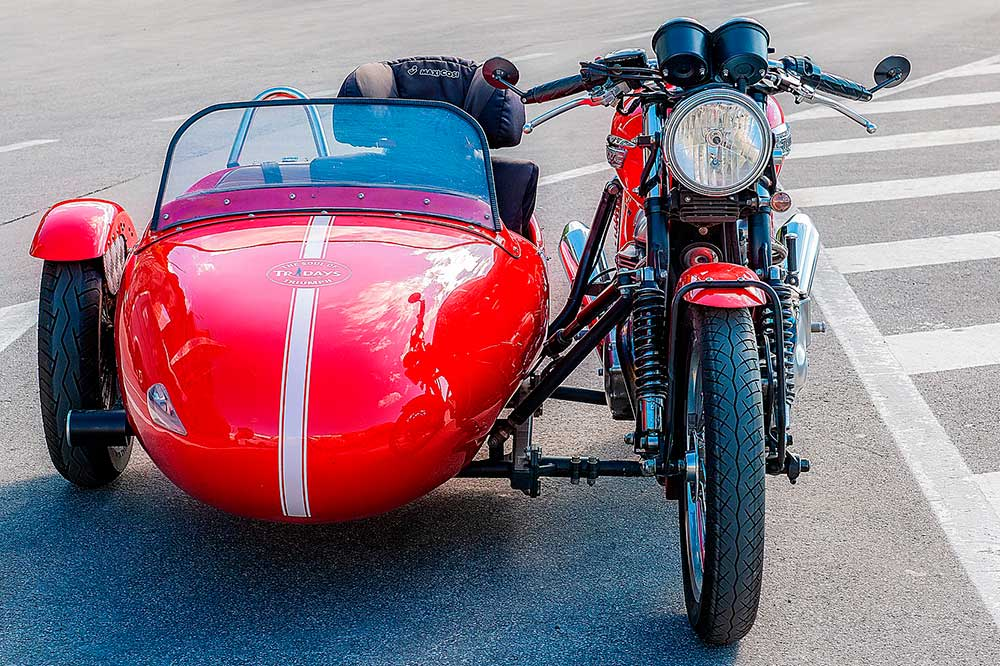
\includegraphics[width=0.9\linewidth]{Images/sidecar}
	\end{figure}
    \begin{figure}
    		\centering
    		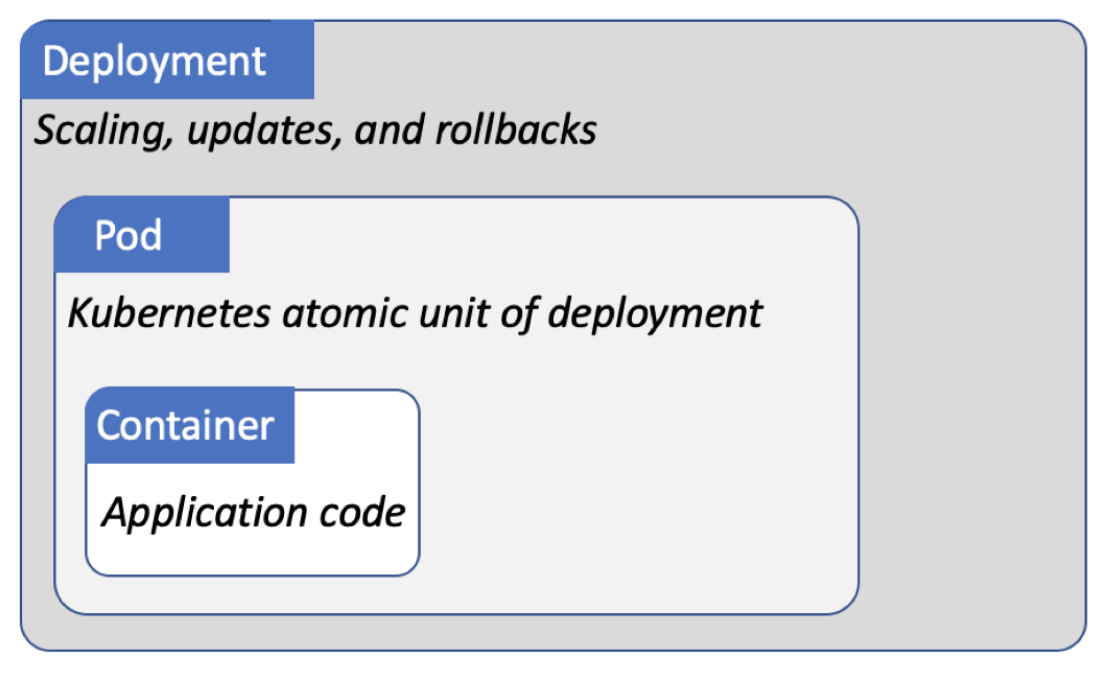
\includegraphics[width=\linewidth]{Images/pod}
    	\end{figure}
\end{column}
\end{columns}


\end{frame}


\begin{frame}{Linkerd}

	\begin{figure}
		\centering
		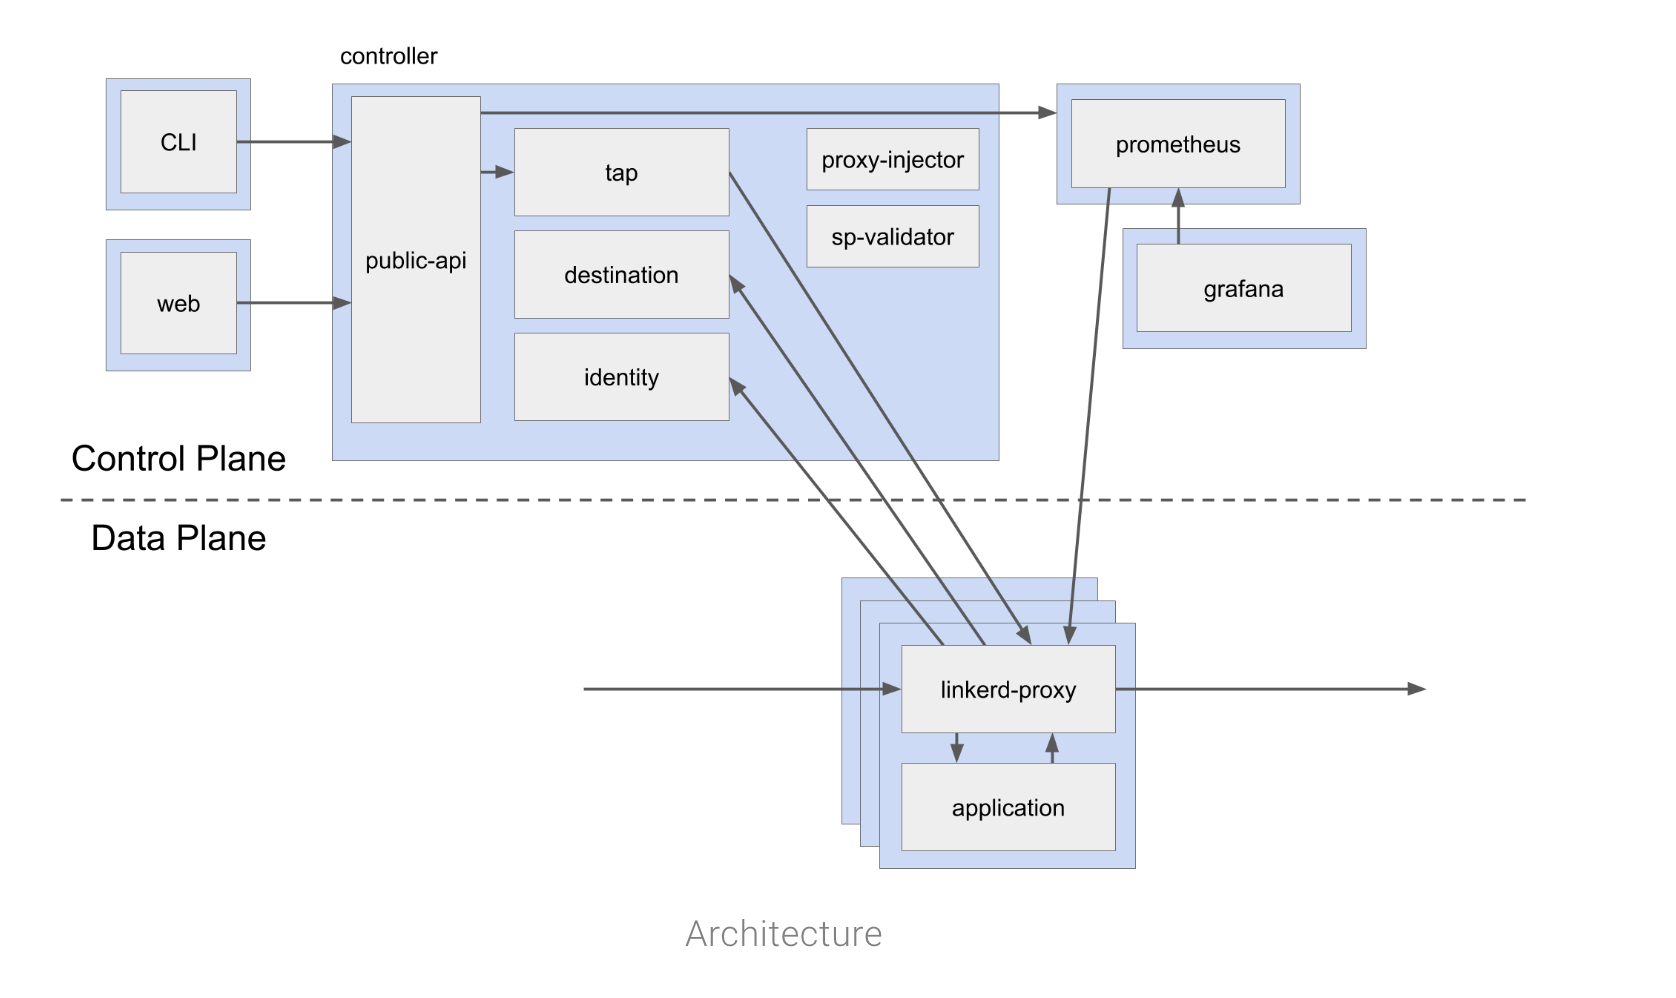
\includegraphics[width=0.9\linewidth]{Images/linkerd.png}
	\end{figure}


\end{frame}


\begin{frame}{Demo!}

	\begin{figure}
		\centering
		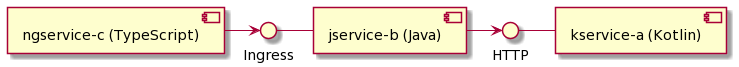
\includegraphics[width=0.9\linewidth]{Images/k8sdemo.png}
	\end{figure}

\url{https://github.com/tuxtor/polyglot-linkerd}

\end{frame}



\begin{frame}{Víctor Orozco}
\begin{columns}[T] % contents are top vertically aligned

	\begin{column}[T]{4cm} % alternative top-align that's better for graphics
		\begin{figure}
			\centering
			
\includegraphics[width=\linewidth]{Images/logos}
		\end{figure}
	\end{column}
	\begin{column}[T]{6cm} % each column can also be its own environment
		\begin{itemize}
			\item vorozco@nabenik.com
			\item \href{https://twitter.com/tuxtor}{@tuxtor}
			\item \href{https://vorozco.com}{https://vorozco.com}
			\item \href{https://tuxtor.shekalug.org}{https://tuxtor.shekalug.org}
		\end{itemize}
		\begin{center}
			
\includegraphics[width=0.1\linewidth]{Images/cclogo}
			\\
			This work is licensed under Creative Commons Attribution-NonCommercial-ShareAlike 3.0 Guatemala (CC BY-NC-SA 3.0 GT).
		\end{center}
	\end{column}
\end{columns}
\end{frame}


\end{document}

